\documentclass[10pt]{article}
\usepackage[paperheight=0.95in,paperwidth=7.2in,margin=0.01in]{geometry}

\usepackage{setspace}
\usepackage{amsmath,amssymb}
\usepackage{amsthm}
\usepackage{fancybox}
\usepackage{url}
\usepackage{enumitem}
\usepackage{multirow}
\usepackage{color}
\usepackage{graphicx}
\usepackage{comment}
\usepackage{bm}
\usepackage{mathtools}
\mathtoolsset{showonlyrefs=true}

\usepackage{multirow}

\usepackage{natbib}
\usepackage{xr}

\input macros.tex
\def\sign{\textup{sgn}}
\usepackage{algpseudocode,algorithm}
\def\sign{\textup{sgn}}
\def\srank{\textup{srank}}
\def\rank{\textup{rank}}
\def\caliP{\mathscr{P}_{\textup{sgn}}}
\def\risk{\textup{Risk}}

\usepackage[table, dvipsnames]{xcolor}


\begin{document}

\renewcommand{\arraystretch}{1}

\begin{table}
\begin{tabular}{c|cccccccc}
Simulation &Signal Tensor $\Theta$ & Rank&  Sign Rank  & Global $\alpha $&CDF of Tensor Entries & Noise  \\
\hline
1&$\tC\times\mM_1\times\mM_2\times\mM_3$ &$3^3$&2& $\infty$& \multirow{4}{*}{
% \begin{minipage}{.2\textwidth}
% \centering
%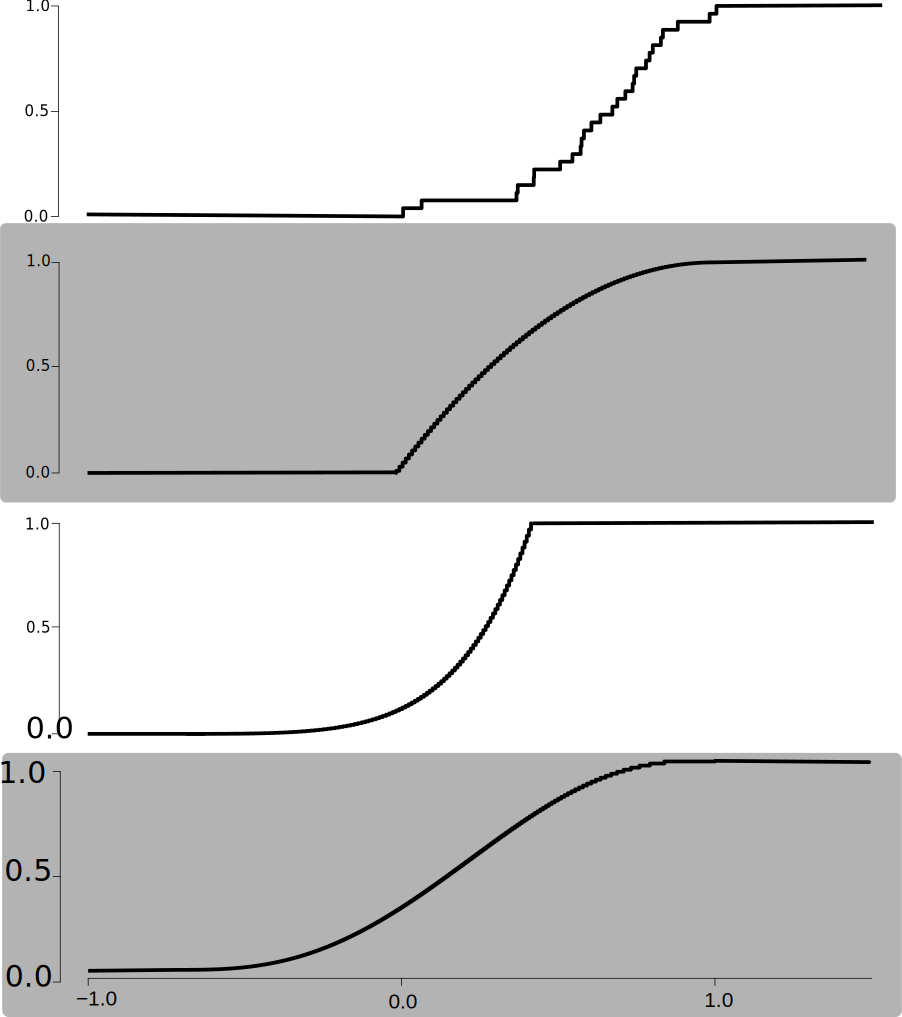
\includegraphics[width=30mm,height=17mm]{cdf_combine_2.pdf}
%  \end{minipage}
}
 &
Uniform $[-0.3,0.3]$\\
  \rowcolor{lightgray}
2& $|\ma\otimes \mathbf{1}\otimes\mathbf{1}-\mathbf{1}\otimes\ma\otimes \mathbf{1}|$& $d$&2&$1$&&
Normal $\tN(0,0.15)$\\
3& $\log(0.5+Z_{\max})$&$\geq d$& 2& 1&&
Uniform $[-0.1,0.1]$\\
 \rowcolor{lightgray}
4& $2.5-\exp(\tZ^{1/3}_{\min})$& $\geq d$ & 2 & 1 & &
Normal $\tN(0,0.15)$
 % \\
%5 &$(1+\exp(\tZ_{\max}+\tZ_{\min}))^{-1}$&$\geq d$&unknown&
%\begin{minipage}{.4\textwidth}
%\centering
%\includegraphics[width=0.3\textwidth,height=6mm]{cdf_Model4.pdf}
 % \end{minipage}
\end{tabular}
\end{table}


\end{document}